\section{Introduction}
\label{sec:intro}

A robot that follows open instructions must ground language in what it sees and act on it. Multimodal LLM (MLLM)
agents do so by giving one model every role: at each step it reads the image and the text history, infers where
the target is, and writes the next actions~\cite{yang2025embodiedbench}. Their success tracks model size. On
EB-Navigation, GPT-4o succeeds in 57.7\% of the episodes and InternVL3-78B in 53.7\%, while models of 7--8B reach
20.3--29.3\% overall and 0--5\% on the Long-horizon subset, in which the target starts behind the agent; a tenfold
larger model of the same family adds \nScaleQwen--\nScaleIntern\,pp. Yet the small models are the ones a robot can
run on board or on a consumer GPU, so the scaling curve seems to rule them out.

Existing remedies leave the model in charge. Training-free agents surround it with memory, reflection, skill
libraries, scene graphs, or tools~\cite{lee2026emho,ma2026brainmem,zhou2026enabling,huang2025esca,ju2026embodiskill},
but the model still writes the plan, and the reported gains rely on 8B to frontier-scale models. Fine-tuned 4B
agents~\cite{xie2026sva,jang2026musix} require training and remain below 60\%. Modular object-navigation systems keep
a metric map~\cite{gadre2022cows,yokoyama2023vlfm,yin2024online} but depend on dedicated detectors.

\begin{figure*}[t]
\centering
\definecolor{oBlueL}{HTML}{DEEBF7}\definecolor{oBlueD}{HTML}{2E75B6}\definecolor{oOrangeP}{HTML}{FDF2E9}\definecolor{oOrangeL}{HTML}{FBE5D6}\definecolor{oOrangeD}{HTML}{C55A11}\definecolor{oOrangeS}{HTML}{ED7D31}\definecolor{oGreenS}{HTML}{C5E0B4}\definecolor{oGreyP}{HTML}{F2F2F2}\definecolor{oGreyL}{HTML}{E7E6E6}\definecolor{oGreyM}{HTML}{BFBFBF}\definecolor{oGreyS}{HTML}{A6A6A6}\definecolor{oGreyK}{HTML}{7F7F7F}\definecolor{oGreyD}{HTML}{595959}
\begin{tikzpicture}[x=1mm, y=1mm, >={Stealth[length=1.4mm, width=1.3mm]}]
\useasboundingbox (0,0) rectangle (174.00,-77.00);
\draw[draw=oGreyK, line width=0.36pt, dash pattern=on 3.2pt off 2.2pt, rounded corners=5pt] (27.64,-30.00) rectangle (53.58,-72.00);
\draw[fill=oOrangeP, draw=oOrangeD, line width=0.8pt, dash pattern=on 3.2pt off 2.2pt, rounded corners=5pt] (59.22,-30.00) rectangle (124.81,-72.00);
\draw[draw=oGreyK, line width=0.36pt, dash pattern=on 3.2pt off 2.2pt, rounded corners=5pt] (130.45,-30.00) rectangle (154.39,-72.00);
\draw[->, line width=0.6pt, draw=black] (11.00,-9.40) -- (16.64,-9.40);
\draw[->, line width=0.6pt, draw=black] (41.64,-9.40) -- (47.29,-9.40);
\draw[->, line width=0.6pt, draw=black] (68.29,-9.40) -- (73.93,-9.40);
\draw[->, line width=0.6pt, draw=black] (99.93,-9.40) -- (160.00,-9.40);
\draw[->, line width=0.6pt, draw=black] (167.00,-14.06) -- (167.00,-18.20) -- (29.14,-18.20) -- (29.14,-14.06);
\draw[->, line width=0.6pt, draw=black] (22.00,-41.06) -- (30.11,-41.06);
\draw[->, line width=0.6pt, draw=oBlueD] (40.61,-45.71) -- (40.61,-48.89);
\draw[->, line width=0.6pt, draw=black] (51.11,-53.54) -- (56.40,-53.54) -- (56.40,-35.07) -- (61.69,-35.07);
\draw[->, line width=0.6pt, draw=oOrangeD] (75.19,-38.14) -- (75.19,-41.31);
\draw[->, line width=0.6pt, draw=oOrangeD] (75.19,-50.63) -- (75.19,-53.80);
\draw[->, line width=0.6pt, draw=oOrangeD] (88.69,-45.97) -- (94.34,-45.97);
\draw[->, line width=0.6pt, draw=black] (122.34,-41.00) -- (132.92,-41.00);
\draw[->, line width=0.6pt, draw=oGreyD] (142.42,-44.07) -- (142.42,-47.24);
\draw[->, line width=0.6pt, draw=black] (151.92,-51.90) -- (160.00,-51.90);
\draw[->, line width=0.6pt, draw=black] (167.00,-56.56) -- (167.00,-75.00) -- (11.00,-75.00) -- (11.00,-58.40);
\node[font=\rmfamily\fontsize{8.5}{10.20}\selectfont, text width=70.00mm, align=left, inner sep=0, anchor=west] at (0.00,-1.80) {\textbf{(a)\ EB prompt (benchmark agent)}};
\node[inner sep=0, anchor=north west] at (0.00,-3.90) {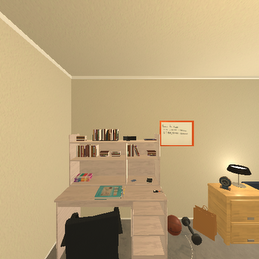
\includegraphics[width=11.00mm, height=11.00mm]{fig/arch_ebframe.png}};
\draw[black, line width=0.19pt] (0.00,-3.90) rectangle (11.00,-14.90);
\filldraw[fill=oGreyL, draw=black, line width=0.36pt, rounded corners=2.6pt] (16.64,-4.74) rectangle (41.64,-14.06);
\node[font=\rmfamily\fontsize{7.5}{9.00}\selectfont, text width=20.06mm, align=center, inner sep=0, anchor=center] at (29.14,-9.40) {instruction $\ell$,\\examples, log $h_t$};
\filldraw[fill=oBlueL, draw=black, line width=0.36pt, rounded corners=2.6pt] (47.29,-4.74) rectangle (68.29,-14.06);
\node[font=\rmfamily\fontsize{7.5}{9.00}\selectfont, text width=16.06mm, align=center, inner sep=0, anchor=center] at (57.79,-9.40) {VLM $f$\\[-0.2mm]{\fontsize{6.5}{7}\selectfont\itshape frozen}};
\filldraw[fill=oGreyL, draw=black, line width=0.36pt, rounded corners=2.6pt] (73.93,-4.74) rectangle (99.93,-14.06);
\node[font=\rmfamily\fontsize{7.5}{9.00}\selectfont, text width=21.06mm, align=center, inner sep=0, anchor=center] at (86.93,-9.40) {text plan of\\action ids};
\filldraw[fill=oGreenS, draw=black, line width=0.36pt, rounded corners=2.6pt] (160.00,-4.74) rectangle (174.00,-14.06);
\node[font=\rmfamily\fontsize{7.5}{9.00}\selectfont, text width=9.06mm, align=center, inner sep=0, anchor=center] at (167.00,-9.40) {actions\\$u_{t:t+m}$};
\node[font=\rmfamily\fontsize{6.5}{7.80}\selectfont\itshape, text width=52.07mm, align=center, inner sep=0, anchor=center] at (129.97,-6.70) {spatial state only in generated text};
\fill[white] (118.00,-16.95) rectangle (134.00,-19.45);
\node[font=\rmfamily\fontsize{7.0}{8.40}\selectfont, text width=16.00mm, align=center, inner sep=0, anchor=center] at (126.00,-18.20) {feedback};
\node[font=\rmfamily\fontsize{8.5}{10.20}\selectfont, text width=70.00mm, align=left, inner sep=0, anchor=west] at (0.00,-22.80) {\textbf{(b)\ \ours (ours)}};
\node[font=\rmfamily\fontsize{8.5}{10.20}\selectfont\bfseries\itshape, text width=25.34mm, align=left, inner sep=0, anchor=west] at (28.24,-27.60) {Per-image questions};
\node[font=\rmfamily\fontsize{8.5}{10.20}\selectfont\bfseries\itshape, text width=64.98mm, align=left, inner sep=0, anchor=west] at (59.82,-27.60) {Metric hypothesis memory};
\node[font=\rmfamily\fontsize{8.5}{10.20}\selectfont\bfseries\itshape, text width=27.94mm, align=left, inner sep=0, anchor=west] at (131.05,-27.60) {Search and control};
\node[font=\rmfamily\fontsize{7.0}{8.40}\selectfont, text width=22.00mm, align=center, inner sep=0, anchor=center] at (11.00,-32.60) {frame $I_t$,\\phrase $s$};
\node[inner sep=0, anchor=north west] at (0.00,-36.40) {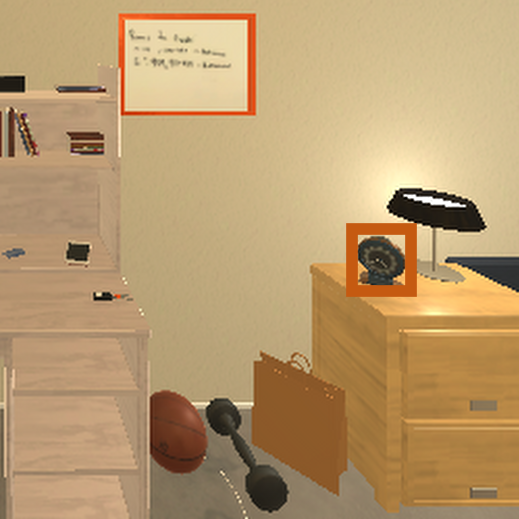
\includegraphics[width=22.00mm, height=22.00mm]{fig/arch_frame.png}};
\draw[black, line width=0.19pt] (0.00,-36.40) rectangle (22.00,-58.40);
\filldraw[fill=oBlueL, draw=black, line width=0.36pt, rounded corners=2.6pt] (30.11,-36.40) rectangle (51.11,-45.71);
\node[font=\rmfamily\fontsize{7.5}{9.00}\selectfont, text width=16.06mm, align=center, inner sep=0, anchor=center] at (40.61,-41.06) {VLM $f$\\[-0.2mm]{\fontsize{6.5}{7}\selectfont\itshape frozen}};
\filldraw[fill=oGreyP, draw=black, line width=0.36pt, rounded corners=2.6pt] (30.11,-48.89) rectangle (51.11,-58.20);
\node[font=\rmfamily\fontsize{7.5}{9.00}\selectfont, text width=16.06mm, align=center, inner sep=0, anchor=center] at (40.61,-53.54) {presence $\pi_t$\\box $b_t$};
\filldraw[fill=oOrangeL, draw=black, line width=0.36pt, rounded corners=2.6pt] (61.69,-32.00) rectangle (88.69,-38.14);
\node[font=\rmfamily\fontsize{7.5}{9.00}\selectfont, text width=22.06mm, align=center, inner sep=0, anchor=center] at (75.19,-35.07) {lift with $D_t$, $p_t$};
\filldraw[fill=oOrangeL, draw=black, line width=0.36pt, rounded corners=2.6pt] (61.69,-41.31) rectangle (88.69,-50.63);
\node[font=\rmfamily\fontsize{7.5}{9.00}\selectfont, text width=22.06mm, align=center, inner sep=0, anchor=center] at (75.19,-45.97) {fuse viewpoints,\\negative evidence};
\node[inner sep=0, anchor=north west] at (61.69,-53.80) {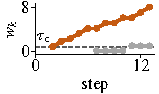
\includegraphics[width=27.00mm, height=16.20mm]{fig/arch_evidence.pdf}};
\node[inner sep=0, anchor=north west] at (94.34,-32.00) {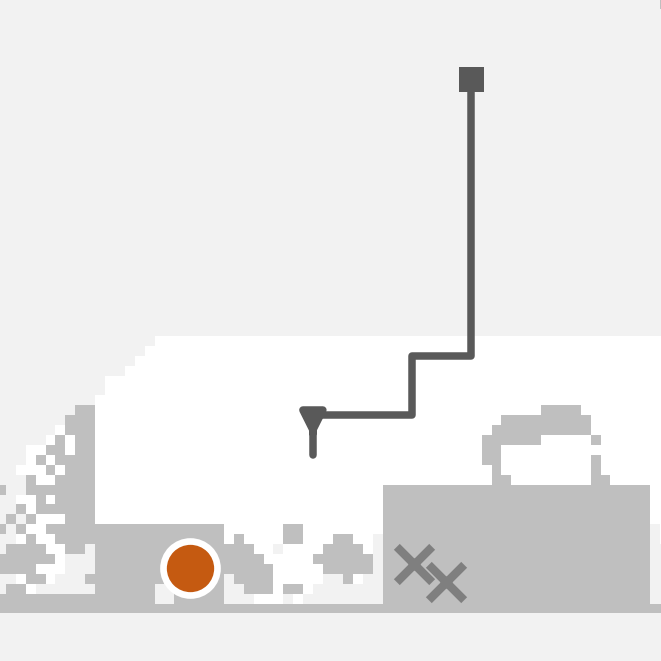
\includegraphics[width=28.00mm, height=28.00mm]{fig/arch_bev.png}};
\draw[black, line width=0.19pt] (94.34,-32.00) rectangle (122.34,-60.00);
\node[font=\rmfamily\fontsize{7.0}{8.40}\selectfont, text width=28.00mm, align=center, inner sep=0, anchor=center] at (108.34,-63.80) {hypotheses $\mu_k$\\on the map $M_t$};
\filldraw[fill=oOrangeL, draw=black, line width=0.36pt, rounded corners=2.6pt] (132.92,-37.93) rectangle (151.92,-44.07);
\node[font=\rmfamily\fontsize{7.5}{9.00}\selectfont, text width=14.06mm, align=center, inner sep=0, anchor=center] at (142.42,-41.00) {select $k^\star$};
\filldraw[fill=oGreyL, draw=black, line width=0.36pt, rounded corners=2.6pt] (132.92,-47.24) rectangle (151.92,-56.56);
\node[font=\rmfamily\fontsize{7.5}{9.00}\selectfont, text width=14.06mm, align=center, inner sep=0, anchor=center] at (142.42,-51.90) {A* planner\\on $M_t$};
\filldraw[fill=oGreenS, draw=black, line width=0.36pt, rounded corners=2.6pt] (160.00,-47.24) rectangle (174.00,-56.56);
\node[font=\rmfamily\fontsize{7.5}{9.00}\selectfont, text width=9.06mm, align=center, inner sep=0, anchor=center] at (167.00,-51.90) {action\\$u_t$};
\fill[white] (76.00,-73.75) rectangle (104.00,-76.25);
\node[font=\rmfamily\fontsize{7.0}{8.40}\selectfont, text width=28.00mm, align=center, inner sep=0, anchor=center] at (90.00,-75.00) {next frame};
\end{tikzpicture}
\caption{\textbf{(a)}~The EB prompt maps $I_t$, the instruction $\ell$, and the history $h_t$ to a text plan $u_{t:t+m}$ with the VLM $f$. \textbf{(b)}~\ours asks $f$ for the presence $\pi_t$ and box $b_t$ of the phrase $s$, lifts them with depth $D_t$ and pose $p_t$ into hypotheses $\mu_k$ with evidence $w_k$, selects $k^\star$, and plans $u_t$ on the map $M_t$. Blue: the frozen VLM; orange: \ours's memory. Thumbnails: one Long-horizon test episode, with the VLM's box on the target, the evidence of the target (orange) passing the commit threshold $\tau_c$ while two look-alikes (grey) fall below zero, and the map with the path, the target (orange), and the look-alikes ($\times$).}
\label{fig:arch}
\end{figure*}


We first ask what breaks when a small VLM drives the agent. Motion planning does not: a geometric planner given the
target position solves \nOracle\% of the test episodes. Recognition is imperfect but usable: Qwen3-VL-4B boxes a
visible named target in \nProbeThreeCommon--\nProbeThreeBase\% of single views. The failure lies in the role the model is
given. Asked for a plan at every step, it must carry where the target was and which way it faces through generated
text (\cref{fig:arch}a), and nothing checks this text against the world. Prompted agents therefore lose targets
they have seen, collide with furniture, and never turn toward a target behind them (\cref{sec:diagnosis}).

A small VLM is thus a good semantic sensor and a poor state keeper, so we build the agent around the model rather
than inside it. \ours (Semantic-to-Metric, \cref{fig:arch}b) is a training-free navigation agent with three parts.
\emph{Perception} asks the VLM two questions per frame, whether the target is visible and where it is in the image,
and checks a magnified crop only when the answer is weak. \emph{Memory} lifts each answer with depth and pose into
a metric target hypothesis, accumulates evidence only from distinct viewpoints, and discards a hypothesis that
reaching it shows to be a look-alike. \emph{Action} commits to a confident hypothesis, inspects a weak one in view,
and otherwise looks around and explores; an occupancy-map planner computes every move. Each part
removes one diagnosed failure: the memory keeps a seen target, the map prevents collisions, and the look-around
finds a target behind the agent.

\begin{figure}[t]
\centering
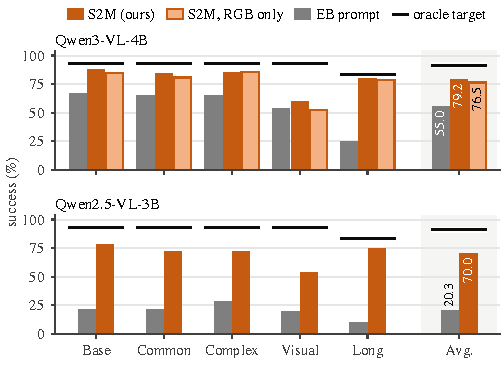
\includegraphics[width=\linewidth]{fig/results.pdf}
\caption{EB-Navigation test success with the same local model (60 episodes per subset). Black line: geometric
planner given the true target position (oracle target). The RGB-only configuration was run with Qwen3-VL-4B.}
\label{fig:results}
\end{figure}

Changing the model's role moves it further than scaling it (\cref{fig:results}), with the profile that the
diagnosis predicts. With Qwen3-VL-4B at 4-bit, \ours succeeds in \nSThree\% of the EB-Navigation test episodes,
${+}\nGainThree$\,pp over the benchmark's agent with the same model, as much as the tenfold scale-up from
InternVL3-8B to 78B gives, and it closes \nGapClosed\% of the gap to the oracle planner. On the Long-horizon subset
it solves \nSThreeLong\% against \nEBThreeLong\%, above every reported agent but one tool-augmented GPT-4o. Each step
takes \nSecS\,s instead of \nSecEB\,s, because the model answers two short questions instead of writing a plan. With
Qwen2.5-VL-3B~\cite{bai2025qwen25vl} the gain grows to ${+}\nGainTwo$\,pp, and on RoboTHOR
ObjectNav~\cite{deitke2020robothor}, which requires an explicit stop, \ours reaches \nRoboSR\% zero-shot.

\noindent\textbf{Contributions.}
\makeatletter\@beginparpenalty=10000\makeatother
\begin{itemize}\setlength{\itemsep}{1pt}\setlength{\parskip}{0pt}\setlength{\leftmargin}{1em}
\item \textbf{Diagnosis.} Small VLMs fail as navigation agents because they must keep spatial state in text, not
because they cannot recognize the target or plan a path.
\item \textbf{The VLM as a sensor, not a planner.} \ours inverts the control of MLLM agents: a metric controller
asks the VLM only questions that the current image can settle, and the VLM never sees the history, the map, or the
plan.
\item \textbf{Evidence fusion for a generative sensor.} A metric hypothesis memory accumulates the model's
presence and box answers over distinct viewpoints and discards look-alikes on arrival, turning unreliable
single answers into a stable target; a modular agent that acts on single-view answers of the same model trails \ours by
\nSOverMod\,pp.
\item \textbf{RGB-only operation.} A per-frame ground-plane scale for monocular depth raises RGB-only success from
\nRGBGlobal\% to \nRGBThree\%, within \nGapRGBAbs\,pp of a depth sensor.
\item \textbf{Results.} On the full EB-Navigation and RoboTHOR splits, a 4-bit 4B model without training and from RGB
alone outperforms GPT-4o, both fine-tuned 4B agents, and \nNTrainFreeBelowRGB{} of \nNTrainFree{} training-free agents
built on 8B to frontier-scale models, and it loses \nScaleDrop\,pp when the model shrinks to 3B, where the benchmark's
agent loses \nScaleDropEB\,pp.
\end{itemize}
